\chapter{Experiments and Results}

This chapter presents our experimental findings across all eight benchmarks and three model scales.

\section{Main Results}

Table~\ref{tab:main_results} presents the consolidated accuracy across all benchmarks, models, and reasoning strategies.

\begin{table}[ht]
\centering
\small
\setlength{\tabcolsep}{2.5pt}
\begin{tabular}{lcccc|cccc|cccc}
\toprule
\multirow{2}{*}{Dataset}
& \multicolumn{4}{c}{LLaMA-3.1-8B}
& \multicolumn{4}{c}{Qwen-0.5B}
& \multicolumn{4}{c}{Qwen-2.5-14B} \\
\cmidrule(lr){2-5} \cmidrule(lr){6-9} \cmidrule(lr){10-13}
& CoT & A* & SC & ToT & CoT & A* & SC & ToT & CoT & A* & SC & ToT \\
\midrule
\multicolumn{13}{c}{\textit{QA Benchmarks}} \\
\midrule
StrategyQA & 64.52 & \textbf{74.80} & 71.22 & 72.24 & 53.60 & 53.40 & \textbf{54.21} & 52.24 & 76.02 & 75.56 & \textbf{80.06} & 78.17 \\
LogicQA & 45.78 & 44.85 & 46.10 & \textbf{46.21} & \textbf{24.00} & 20.20 & 22.10 & 21.19 & 57.91 & 58.12 & \textbf{59.19} & 55.12 \\
HotpotQA & 76.80 & \textbf{80.10} & 78.21 & 78.45 & 8.40 & \textbf{30.00} & 12.21 & 22.17 & 60.19 & \textbf{83.33} & 65.25 & 72.14 \\
\midrule
\multicolumn{13}{c}{\textit{Math Benchmarks}} \\
\midrule
GSM8K & 85.04 & 86.12 & \textbf{86.90} & 60.00 & 26.84 & 14.48 & \textbf{43.22} & 41.02 & 61.56 & \textbf{80.59} & 50.57 & 48.82 \\
MATH & 78.00 & 79.10 & \textbf{79.50} & 40.10 & 32.80 & 16.20 & 41.60 & \textbf{49.00} & 44.00 & \textbf{47.20} & 9.80 & 21.20 \\
\midrule
\multicolumn{13}{c}{\textit{Code Generation}} \\
\midrule
HumanEval & 67.48 & 64.42 & 65.03 & \textbf{71.78} & \textbf{33.74} & 20.25 & 26.38 & 33.13 & 77.91 & 76.07 & 76.07 & \textbf{79.75} \\
MBPP & \textbf{39.80} & 36.80 & 38.00 & 40.40 & \textbf{24.00} & 20.80 & 21.40 & 23.00 & 46.60 & 45.00 & 46.80 & \textbf{49.80} \\
CodeContests & \textbf{100.00} & 87.00 & 99.00 & 91.20 & 49.80 & \textbf{68.20} & 48.80 & 67.80 & \textbf{99.60} & 94.40 & 98.20 & 94.00 \\
\bottomrule
\end{tabular}
\caption{Consolidated results across all benchmarks. Bold indicates the best method per dataset-model combination. No single strategy dominates: A* leads on HotpotQA and GSM8K at larger scales, while CoT/SC/ToT are competitive or better on other tasks.}
\label{tab:main_results}
\end{table}

Key observations:
\begin{itemize}
\item No single strategy uniformly dominates across all datasets and scales.
\item A* provides the largest gains on HotpotQA (multi-hop) and GSM8K at 14B (+19pp over CoT).
\item At 0.5B, A* massively outperforms CoT on CodeContests (+18.4pp) and HotpotQA (+21.6pp).
\item ToT is strongest on HumanEval (code with rich specifications).
\item SC hurts at 0.5B on math and code (model too weak for meaningful majority voting).
\end{itemize}

\begin{figure}[htbp]
\centering
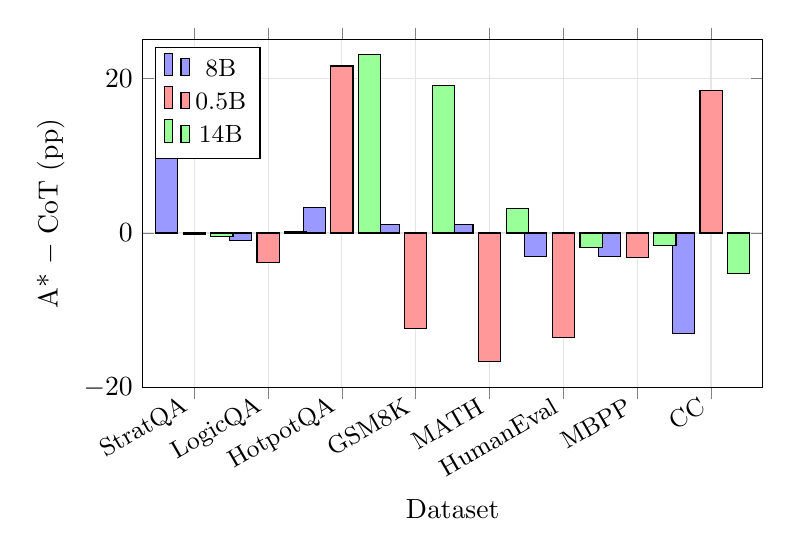
\begin{tikzpicture}
\begin{axis}[
    ybar,
    width=0.78\textwidth,
    height=6cm,
    bar width=8pt,
    xlabel={Dataset},
    ylabel={A* $-$ CoT (pp)},
    symbolic x coords={StratQA, LogicQA, HotpotQA, GSM8K, MATH, HumanEval, MBPP, CC},
    xtick=data,
    x tick label style={rotate=30, anchor=east, font=\small},
    ymin=-20, ymax=25,
    grid=major,
    grid style={gray!20},
    legend style={at={(0.02,0.98)}, anchor=north west, font=\small},
    nodes near coords style={font=\tiny},
]
\addplot[fill=blue!40] coordinates {
    (StratQA, 10.28) (LogicQA, -0.93) (HotpotQA, 3.30) (GSM8K, 1.08) (MATH, 1.10) (HumanEval, -3.06) (MBPP, -3.00) (CC, -13.00)
};
\addplot[fill=red!40] coordinates {
    (StratQA, -0.20) (LogicQA, -3.80) (HotpotQA, 21.60) (GSM8K, -12.36) (MATH, -16.60) (HumanEval, -13.49) (MBPP, -3.20) (CC, 18.40)
};
\addplot[fill=green!40] coordinates {
    (StratQA, -0.46) (LogicQA, 0.21) (HotpotQA, 23.14) (GSM8K, 19.03) (MATH, 3.20) (HumanEval, -1.84) (MBPP, -1.60) (CC, -5.20)
};
\legend{8B, 0.5B, 14B}
\end{axis}
\end{tikzpicture}
\caption{A* advantage over CoT (percentage points) across all datasets and scales. Positive values indicate A* is better; negative indicates CoT is better. The pattern varies substantially by dataset and scale, motivating adaptive routing.}
\label{fig:astar_advantage}
\end{figure}

\FloatBarrier
\section{Instance-Level Complementarity}

Table~\ref{tab:complementarity_thesis} quantifies the instance-level disagreement between CoT and A*.

\begin{table}[ht]
\centering
\small
\begin{tabular}{lcccc}
\toprule
\textbf{Dataset} & \textbf{Both correct} & \textbf{CoT only} & \textbf{A* only} & \textbf{Both wrong} \\
\midrule
StrategyQA (8B) & 59.4\% & 14.3\% & 10.8\% & 15.4\% \\
LogicQA (8B) & 27.6\% & 18.1\% & 13.5\% & 40.7\% \\
HotpotQA (8B) & 59.6\% & 17.2\% & 17.4\% & 5.8\% \\
\midrule
HumanEval (8B) & 57.1\% & 10.4\% & 7.4\% & 25.2\% \\
MBPP (8B) & 32.6\% & 7.2\% & 4.2\% & 56.0\% \\
CodeContests (0.5B) & 42.0\% & 7.8\% & 26.2\% & 24.0\% \\
\bottomrule
\end{tabular}
\caption{Instance-level complementarity. The ``CoT only'' and ``A* only'' columns show substantial non-overlap, confirming that a router can improve over either fixed strategy.}
\label{tab:complementarity_thesis}
\end{table}

The oracle gaps are substantial: +9.79pp on StrategyQA, +14.10pp on HotpotQA, and the CodeContests 0.5B oracle reaches 76.0\% vs. best single at 68.2\%.

\FloatBarrier
\section{Topology Cluster Analysis}

Applying $k$-means ($k=4$) to the 13 topology features across QA/math instances yields four interpretable clusters (Table~\ref{tab:clusters_thesis}).

\begin{table}[ht]
\centering
\small
\begin{tabular}{llcccl}
\toprule
\textbf{Cluster} & \textbf{Profile} & \textbf{BC} & \textbf{A*\%} & \textbf{CoT\%} & \textbf{Interpretation} \\
\midrule
C1 & Linear, short & 1.28 & 81.7 & 82.1 & CoT sufficient \\
C2 & Mid-branch & 4.24 & 73.5 & 66.2 & Routing critical \\
C3 & Complex, noisy & 4.02 & 52.3 & 49.1 & Both often fail \\
C4 & Deep-branch & 6.49 & 69.8 & 58.4 & A* largest gain \\
\bottomrule
\end{tabular}
\caption{Topology clusters. BC = branching coefficient. A* advantage grows monotonically with branching complexity ($R^2 = 0.94$).}
\label{tab:clusters_thesis}
\end{table}

\begin{figure}[htbp]
\centering
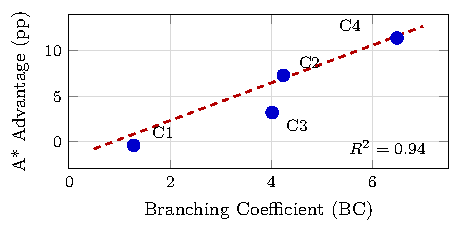
\includegraphics[width=0.65\textwidth]{topology_scatter.pdf}
\caption{A* advantage (pp) vs. branching coefficient across topology clusters. The linear fit ($R^2 = 0.94$) shows that branching coefficient is a strong predictor of when search helps.}
\label{fig:topology_scatter_thesis}
\end{figure}

The prescriptive decision rule: C1 (linear) $\rightarrow$ use CoT; C2 (mid-branch) $\rightarrow$ route adaptively; C3 (complex) $\rightarrow$ neither reliable; C4 (deep-branch) $\rightarrow$ use A*.

\FloatBarrier
\section{Router Comparison}

\subsection{8B Scale}

Table~\ref{tab:router_8b_thesis} compares all routing strategies on LLaMA-3.1-8B.

\begin{table}[ht]
\centering
\small
\setlength{\tabcolsep}{3pt}
\begin{tabular}{llccccccccc}
\toprule
\textbf{Router} & \textbf{Input} & \textbf{Str.QA} & \textbf{Log.QA} & \textbf{Hot.QA} & \textbf{GSM8K} & \textbf{MATH} & \textbf{HE} & \textbf{MBPP} & \textbf{CC} & \textbf{Gap\%} \\
\midrule
A* only & traces & 74.80 & 44.85 & 80.10 & 86.12 & 79.10 & 64.42 & 36.80 & 87.00 & $-$10.9 \\
CoT only & traces & 64.52 & 45.78 & 76.80 & 85.04 & 78.00 & 67.48 & 39.80 & 100.00 & $-$24.6 \\
\midrule
Sem.\ Entropy & traces & 74.37 & 47.47 & 81.30 & 86.67 & 78.24 & 65.64 & 37.00 & 88.20 & $-$3.9 \\
LLM-as-Critic & traces & 74.19 & 47.16 & 80.21 & 87.28 & 79.13 & 71.17 & 40.20 & 97.80 & 9.6 \\
LLM-as-Judge & traces & 73.28 & 47.21 & 80.87 & 85.65 & 78.23 & 71.78 & 40.40 & 97.80 & 6.6 \\
Random Forest & features & 76.25 & 48.20 & 81.25 & 87.43 & 80.12 & 67.48 & 39.60 & 100.00 & 11.2 \\
\textbf{Topology} & \textbf{13 feat.} & \textbf{77.35} & \textbf{49.01} & \textbf{82.41} & \textbf{91.10} & \textbf{81.52} & \textbf{72.50} & \textbf{40.63} & \textbf{100.00} & \textbf{32.3} \\
\midrule
Oracle & -- & 84.59 & 59.29 & 94.20 & 96.14 & 84.17 & 74.85 & 44.00 & 100.00 & 100 \\
\bottomrule
\end{tabular}
\caption{Router comparison at 8B. The topology router achieves 32.3\% oracle-gap recovery using only pre-generation features, outperforming all trace-based routers.}
\label{tab:router_8b_thesis}
\end{table}

\subsection{14B and 0.5B Scales}

The topology router maintains its advantage at other scales:
\begin{itemize}
\item \textbf{14B:} Topology achieves 11.9\% gap recovery---the only router with positive recovery (all trace-based routers are negative).
\item \textbf{0.5B:} Topology achieves 25.6\% gap recovery, with 89.7\% recovery on CodeContests alone.
\end{itemize}

\begin{figure}[htbp]
\centering
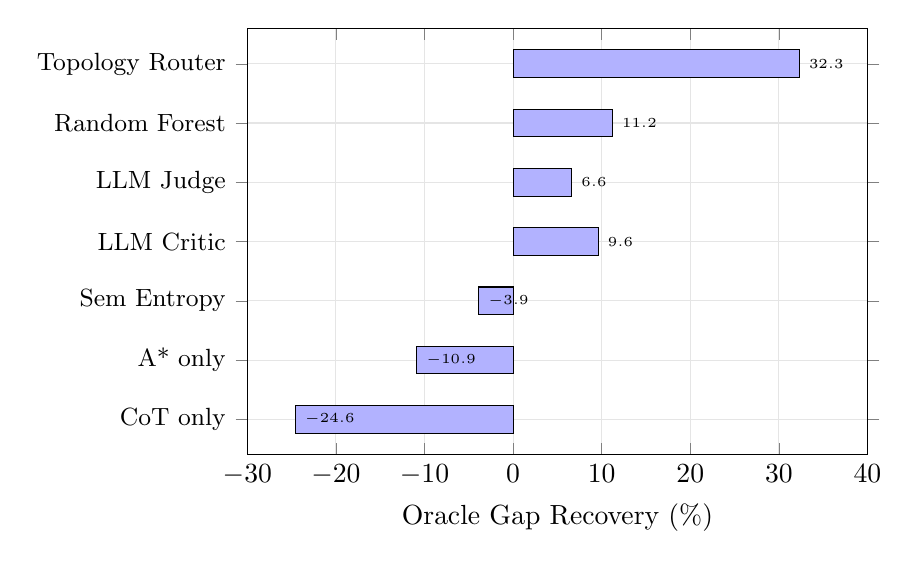
\begin{tikzpicture}
\begin{axis}[
    xbar,
    width=0.78\textwidth,
    height=7cm,
    bar width=10pt,
    xlabel={Oracle Gap Recovery (\%)},
    ylabel={},
    symbolic y coords={CoT only,A* only,Sem Entropy,LLM Critic,LLM Judge,Random Forest,Topology Router},
    ytick=data,
    y tick label style={font=\small},
    xmin=-30, xmax=40,
    grid=major,
    grid style={gray!20},
    nodes near coords,
    nodes near coords style={font=\tiny},
    every node near coord/.append style={anchor=west},
]
\addplot[fill=blue!30] coordinates {
    (-24.6,CoT only)
    (-10.9,A* only)
    (-3.9,Sem Entropy)
    (9.6,LLM Critic)
    (6.6,LLM Judge)
    (11.2,Random Forest)
    (32.3,Topology Router)
};
\end{axis}
\end{tikzpicture}
\caption{Oracle gap recovery at 8B across all benchmarks. Only the topology router achieves substantial positive recovery (32.3\%). Using A* alone or CoT alone yields \emph{negative} recovery (worse than the per-dataset best). Trace-based routers provide modest gains but are limited by the Fluency-Correctness Asymmetry.}
\label{fig:gap_recovery}
\end{figure}

\section{Fluency-Correctness Asymmetry}

We identify why pre-generation routing outperforms post-hoc routing: in 38\% of disagreement cases, CoT produces a more fluent trace but the wrong answer. This systematically misleads any critic or judge that uses readability as a proxy for correctness.

\begin{table}[ht]
\centering
\small
\begin{tabular}{lcc}
\toprule
\textbf{Metric} & \textbf{A*} & \textbf{CoT} \\
\midrule
Average fluency score & 0.725 & 0.673 \\
Cases where more fluent & 62.0\% & 38.0\% \\
More-fluent but wrong & \multicolumn{2}{c}{38.0\% of disagreements} \\
\bottomrule
\end{tabular}
\caption{Fluency-Correctness Asymmetry. The more fluent trace is wrong in 38\% of cases.}
\label{tab:fluency_thesis}
\end{table}

\FloatBarrier
\section{Code Generation Extension}

\subsection{Multi-Return Tasks}

On HumanEval, tasks requiring multi-value returns exhibit a striking scale-dependent interaction:

\begin{table}[ht]
\centering
\small
\begin{tabular}{lccc}
\toprule
\textbf{Scale} & \textbf{CoT (multi-return)} & \textbf{A* (multi-return)} & \textbf{A* advantage} \\
\midrule
0.5B & 45.5\% & 18.2\% & $-$27.3pp \\
8B & 100.0\% & 81.8\% & $-$18.2pp \\
14B & 81.8\% & \textbf{100.0\%} & +18.2pp \\
\bottomrule
\end{tabular}
\caption{Multi-return tasks on HumanEval ($n=11$). A* achieves perfect accuracy only at 14B---a ``capability threshold'' for search.}
\label{tab:multi_return_thesis}
\end{table}

This suggests that A* on structurally complex tasks requires sufficient base-model competence to generate meaningful alternatives.

\begin{figure}[htbp]
\centering
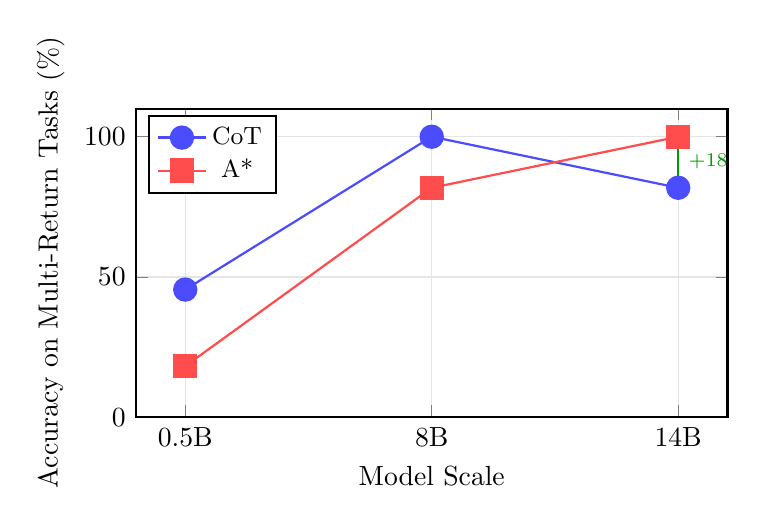
\begin{tikzpicture}
\begin{axis}[
    width=0.75\textwidth,
    height=5.5cm,
    xlabel={Model Scale},
    ylabel={Accuracy on Multi-Return Tasks (\%)},
    symbolic x coords={0.5B, 8B, 14B},
    xtick=data,
    ymin=0, ymax=110,
    grid=major,
    grid style={gray!20},
    legend style={at={(0.02,0.98)}, anchor=north west, font=\small},
    mark size=4pt,
    thick,
]
\addplot[blue!70, mark=*, thick] coordinates {(0.5B, 45.5) (8B, 100.0) (14B, 81.8)};
\addplot[red!70, mark=square*, thick] coordinates {(0.5B, 18.2) (8B, 81.8) (14B, 100.0)};
\legend{CoT, A*}

\draw[<->, thick, green!60!black] (axis cs:14B, 83) -- (axis cs:14B, 99) node[midway, right, font=\scriptsize] {+18.2pp};
\end{axis}
\end{tikzpicture}
\caption{Multi-return task accuracy across scales. At 14B, A* achieves \textbf{perfect accuracy} while CoT drops---a ``capability threshold'' where the model becomes strong enough for search to explore meaningful alternatives. The pattern reverses from 8B (where CoT is perfect).}
\label{fig:multi_return_scaling}
\end{figure}

\subsection{Category Analysis (MBPP)}

\begin{table}[ht]
\centering
\small
\begin{tabular}{lcccc}
\toprule
\textbf{Category} & \textbf{$n$} & \textbf{8B (A* adv.)} & \textbf{14B (A* adv.)} \\
\midrule
String & 93 & +4.3pp & +1.1pp \\
Logic/validation & 60 & $-$1.7pp & +5.0pp \\
Other & 55 & +3.6pp & +1.8pp \\
List operations & 246 & $-$2.4pp & $-$3.3pp \\
Math/numeric & 227 & $-$7.5pp & $-$1.3pp \\
\bottomrule
\end{tabular}
\caption{MBPP by category. A* helps on validation tasks (multiple conditions to check); CoT wins on clear algorithmic transformations.}
\label{tab:categories_thesis}
\end{table}

\subsection{CodeContests: Search Helps Small Models}

At 0.5B, A* provides +18.4pp over CoT on CodeContests (68.2\% vs. 49.8\%), with 26.2\% of instances solved exclusively by A*. This mirrors the HotpotQA pattern and confirms that search is most valuable when the base model cannot reach the solution directly but can generate meaningful candidate steps for the search to select among.

\FloatBarrier
\section{Sensitivity and Compute Analysis}

\subsection{Budget Sweep}

On a 300-question HotpotQA sample, accuracy improves from $B=5$ (73.0\%) to $B=20$ (78.7\%), then drops at $B=30$ (76.0\%), indicating diminishing returns.

\subsection{Compute Cost}

A* at default settings uses $\sim$12,452 tokens/question ($\sim$24$\times$ CoT) on QA, but only 1.7--3.4$\times$ on code tasks (shorter solutions, fewer nodes needed). This makes topology-based routing particularly practical for code.

\begin{figure}[htbp]
\centering
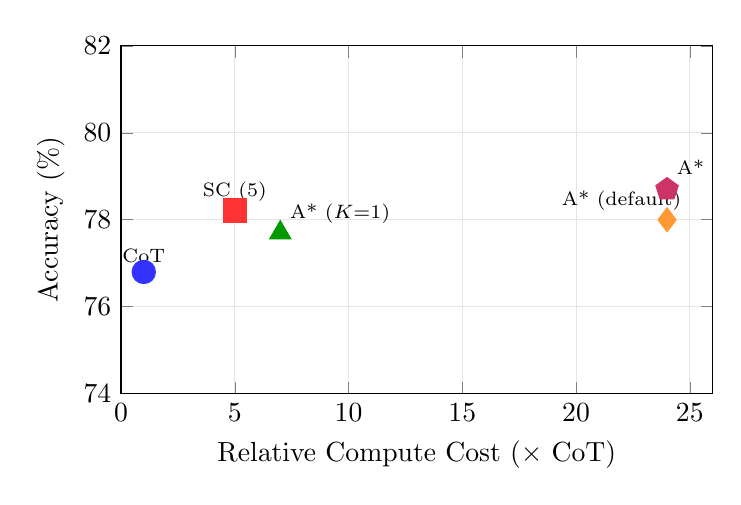
\begin{tikzpicture}
\begin{axis}[
    width=0.75\textwidth,
    height=6cm,
    xlabel={Relative Compute Cost ($\times$ CoT)},
    ylabel={Accuracy (\%)},
    xmin=0, xmax=26,
    ymin=74, ymax=82,
    grid=major,
    grid style={gray!20},
    legend style={at={(0.98,0.02)}, anchor=south east, font=\small},
    mark size=4pt,
]
\addplot[only marks, mark=*, blue!80, thick] coordinates {(1, 76.80)};
\addplot[only marks, mark=square*, red!80, thick] coordinates {(5, 78.21)};
\addplot[only marks, mark=triangle*, green!60!black, thick] coordinates {(7, 77.70)};
\addplot[only marks, mark=diamond*, orange!80, thick] coordinates {(24, 78.00)};
\addplot[only marks, mark=pentagon*, purple!80, thick] coordinates {(24, 78.70)};

\node[font=\scriptsize, anchor=south] at (axis cs:1, 76.80) {CoT};
\node[font=\scriptsize, anchor=south] at (axis cs:5, 78.21) {SC (5)};
\node[font=\scriptsize, anchor=south west] at (axis cs:7, 77.70) {A* ($K$=1)};
\node[font=\scriptsize, anchor=south] at (axis cs:22, 78.00) {A* (default)};
\node[font=\scriptsize, anchor=south west] at (axis cs:24, 78.70) {A* (peak)};

\end{axis}
\end{tikzpicture}
\caption{Compute--accuracy tradeoff on HotpotQA (8B). A* at $K$=1 (no branching) already exceeds SC at lower cost. The topology router avoids the 24$\times$ cost of full A* on instances where CoT suffices, achieving better average accuracy at lower average cost.}
\label{fig:compute_tradeoff}
\end{figure}

\section{Human Evaluation}

Two annotators labeled 100 disagreement instances per dataset on coverage (1--3) and relevance (1--3), with Cohen's $\kappa$: 0.59--0.68. The correct method consistently achieves higher coverage, confirming that disagreements are driven by coverage of the required reasoning path rather than surface quality.

\section{Qualitative Examples}

We present representative examples demonstrating when A* succeeds (multi-constraint problems) and when CoT succeeds (direct algorithmic implementations). Full examples are provided in the appendix of our TMLR submission.

\textbf{A* Success (HumanEval/1 --- separate\_paren\_groups):} The task requires parsing nested parentheses into balanced groups. A* explores multiple parsing strategies (stack-based, counter-based) and selects the correct one. CoT commits to a single approach that fails on space handling.

\textbf{CoT Success (HumanEval/14 --- all\_prefixes):} Return all prefixes of a string. CoT generates a correct one-line list comprehension. A* over-explores and introduces an off-by-one error.
